%%% PREAMBOLO %%%
\documentclass[a4paper, 12pt]{article}

%%% PACCHETTI %%%
% Layout di pagina
\usepackage[a4paper,top=2cm,bottom=2cm,left=3cm,right=3cm,marginparwidth=1.75cm]{geometry}

% Supporto linguistico
\usepackage[utf8]{inputenc}
\usepackage[T1]{fontenc}
\usepackage[italian]{babel}

% Pacchetti per elementi grafici e formattazione
\usepackage{graphicx}
\usepackage{xcolor}
\usepackage{float}

% Tabelle avanzate
\usepackage{booktabs}
\usepackage{makecell}

% Matematica
\usepackage{amsmath}
\usepackage{amssymb}

% Programmazione
\usepackage{listings}

% Supporto per link e PDF
\usepackage{hyperref}
\usepackage{caption}
\usepackage{subcaption}

% Supporto per tabelle e figure
\usepackage{forest}


%%% CONFIGURAZIONI %%%
% Configurazione hyperref
\hypersetup{
    pdftitle={Progetto Tetris Arduino},
    pdfauthor={Enrico Ferraiolo},
    colorlinks=true,
    linkcolor=blue,
    citecolor=green,
    urlcolor=cyan
}

% Definizione comandi personalizzati
\newcommand{\RedBlock}{\colorbox{red}{\rule{1.2ex}{1.2ex}}}      % blocco pieno rosso
\newcommand{\WhiteBlock}{\fcolorbox{black}{white}{\rule{1.2ex}{1.2ex}}} % blocco vuoto

% Impostazione della configurazione listings per il codice
\lstset{
    basicstyle=\ttfamily\small,
    keywordstyle=\color{blue},
    commentstyle=\color{green!50!black},
    stringstyle=\color{red},
    breaklines=true,
    showstringspaces=false
}

%%% INFORMAZIONI SUL DOCUMENTO %%%
\title{\textbf{RELAZIONE: \\ Tetris Arduino}}
\author{Enrico Ferraiolo 0001191698}
\date{}

%%% INIZIO DOCUMENTO %%%
\begin{document}

% Frontespizio
\maketitle

\begin{center}
    \textbf{Laurea Magistrale in Informatica}\\
    \vspace{0.3cm}
    Corso: Laboratorio di Making\\
    a.a. 2024-2025
    \vspace{2cm}
\end{center}

\newpage

% Indice dei contenuti
\tableofcontents
\newpage

%%% CONTENUTO PRINCIPALE %%%
\section{Introduzione}
\label{sec:introduzione}
Il gioco Tetris è uno dei puzzle game più celebri di sempre: l'utente deve ruotare e spostare pezzi geometrici (``tetramini'') che cadono,
completando linee orizzontali per ottenere punti.

L'obiettivo di questo progetto è realizzare una versione giocabile su Arduino di Tetris, utilizzando:
\begin{itemize}
    \item un display a matrice LED 8x8 (MAX7219) per il campo di gioco
    \item un display LCD 16x2 per visualizzare punteggio e stato
    \item un telecomando IR e un encoder rotativo per i controlli
\end{itemize}

Lo scopo del progetto è quindi implementare una versione completamente funzionante del gioco Tetris su Arduino con diversi moduli di input e output.

\section{Componenti Hardware}
\label{sec:componenti-hardware}
Di seguito vengono elencati e descritti i componenti hardware utilizzati per il progetto.

\subsection{Microcontrollore}
\label{subsec:microcontrollore}
Il microcontrollore utilizzato è il \textbf{Elegoo UNO R3}, una scheda equivalente all'Arduino UNO che fornisce tutte le funzionalità necessarie per il progetto.

\subsection{Display a matrice LED - Campo di Gioco}
\label{subsec:display-matrice}
Il display a matrice LED è un modulo \textbf{MAX7219} con configurazione 8x8. Ogni LED della matrice può essere controllato individualmente, consentendo di:
\begin{itemize}
    \item visualizzare il campo di gioco
    \item rappresentare i tetramini in movimento
    \item mostrare le celle occupate
\end{itemize}

Ogni LED rappresenta una singola cella del campo di gioco.

\subsection{Display LCD - Informazioni di Gioco}
\label{subsec:display-lcd}
Per visualizzare informazioni testuali viene utilizzato un display LCD 16x2 (\textbf{LCD 1602}). A schermo vengono mostrati:
\begin{itemize}
    \item \textbf{Punteggio}: punteggio attuale del giocatore
    \item \textbf{Stato}: stato corrente del gioco (in corso, pausa, terminato)
    \item \textbf{Velocità}: velocità di caduta dei tetramini
    \item \textbf{Istruzioni ausiliarie}: informazioni utili per il giocatore
\end{itemize}

\subsection{Controlli}
\label{subsec:controlli}
Il progetto implementa due diversi sistemi di controllo per offrire un'interazione flessibile.

\subsubsection{Controlli Infrarossi}
\label{subsubsec:controlli-ir}
Il telecomando IR consente di inviare istruzioni a distanza tramite segnali infrarossi, decodificati da un apposito ricevitore. I comandi principali sono:

\begin{table}[H]
    \centering
    \caption{Funzioni dei tasti del telecomando IR}
    \label{tab:ir-functions}
    \begin{tabular}{ll}
        \toprule
        \textbf{Tasto} & \textbf{Funzione}                    \\
        \midrule
        POWER          & Accensione/spegnimento del gioco     \\
        FAST BACK      & Movimento del tetramino a sinistra   \\
        FAST FORWARD   & Movimento del tetramino a destra     \\
        PAUSE          & Pausa/ripresa del gioco              \\
        VOL+           & Aumento della velocità di caduta     \\
        VOL-           & Diminuzione della velocità di caduta \\
        \bottomrule
    \end{tabular}
\end{table}

\subsubsection{Encoder Rotativo}
\label{subsubsec:encoder}
L'encoder rotativo offre un controllo analogico della velocità di gioco:
\begin{itemize}
    \item \textbf{Rotazione in senso orario}: aumento della velocità di caduta
    \item \textbf{Rotazione in senso antiorario}: diminuzione della velocità di caduta
\end{itemize}

\section{Il Gioco}
\label{sec:gioco}
Tetris è un puzzle game in cui il giocatore deve manipolare dei tetramini che cadono dall'alto nel campo di gioco. L'obiettivo è:
\begin{itemize}
    \item Ruotare e posizionare i tetramini per completare le righe orizzontali
    \item Quando una riga è completa, essa scompare e il giocatore guadagna punti
    \item Il gioco termina quando i tetramini impilati raggiungono la parte superiore del campo
\end{itemize}

\subsection{Tetramini}
\label{subsec:tetramini}
I tetramini implementati nel gioco sono rappresentati nella Tabella \ref{tab:tetramini}:

\begin{table}[H]
    \centering
    \caption{Rappresentazione dei tetramini}
    \label{tab:tetramini}
    \begin{tabular}{
            >{\bfseries}l   % Nome
            c               % Codici binari
            c               % Dimensioni
            l               % Rappresentazione
        }
        \toprule
        Pezzo & Codici binari                                      & W\(\times\)H & Forma \\
        \midrule
        I     & \makecell{\texttt{0b1111}                                                 \\\texttt{0b0000}\\\texttt{0b0000}\\\texttt{0b0000}}
              & 4\(\times\)1
              & \makecell{\RedBlock\RedBlock\RedBlock\RedBlock}                           \\
        \addlinespace
        J     & \makecell{\texttt{0b0111}                                                 \\\texttt{0b0100}}
              & 3\(\times\)2
              & \makecell{\WhiteBlock\RedBlock\RedBlock\RedBlock                          \\\WhiteBlock\RedBlock\WhiteBlock\WhiteBlock} \\
        \addlinespace
        L     & \makecell{\texttt{0b1110}                                                 \\\texttt{0b0010}}
              & 3\(\times\)2
              & \makecell{\RedBlock\RedBlock\RedBlock\WhiteBlock                          \\\WhiteBlock\RedBlock\WhiteBlock\WhiteBlock} \\
        \addlinespace
        O     & \makecell{\texttt{0b0110}                                                 \\\texttt{0b0110}}
              & 2\(\times\)2
              & \makecell{\WhiteBlock\RedBlock\RedBlock\WhiteBlock                        \\\WhiteBlock\RedBlock\RedBlock\WhiteBlock} \\
        \addlinespace
        S     & \makecell{\texttt{0b0111}                                                 \\\texttt{0b0010}}
              & 3\(\times\)2
              & \makecell{\WhiteBlock\RedBlock\RedBlock\RedBlock                          \\\WhiteBlock\WhiteBlock\RedBlock\WhiteBlock} \\
        \addlinespace
        T     & \makecell{\texttt{0b1100}                                                 \\\texttt{0b0110}}
              & 3\(\times\)2
              & \makecell{\RedBlock\RedBlock\WhiteBlock\WhiteBlock                        \\\WhiteBlock\RedBlock\RedBlock\WhiteBlock} \\
        \addlinespace
        Z     & \makecell{\texttt{0b1110}                                                 \\\texttt{0b1000}}
              & 3\(\times\)2
              & \makecell{\RedBlock\RedBlock\RedBlock\WhiteBlock                          \\\RedBlock\WhiteBlock\WhiteBlock\WhiteBlock} \\
        \bottomrule
    \end{tabular}
\end{table}

\section{Ambienti di Sviluppo}
\label{sec:ambienti}
Il progetto è stato sviluppato per essere eseguibile in due configurazioni:
\begin{itemize}
    \item \textbf{Hardware fisico}: con la scheda Elegoo UNO R3 (o equivalente) e tutti i moduli connessi
    \item \textbf{Simulatore}: per test e sviluppo senza hardware fisico
\end{itemize}

La configurazione dell'ambiente avviene tramite la costante \texttt{PRODUCTION} nel file sorgente principale:
\begin{itemize}
    \item \texttt{PRODUCTION = true}: per l'utilizzo con hardware fisico
    \item \texttt{PRODUCTION = false}: per l'utilizzo con il simulatore
\end{itemize}

Questa differenziazione è necessaria principalmente per gestire i diversi codici infrarossi generati dal telecomando nei due ambienti.

\section{Setup Hardware}
\label{sec:setup}
Questa sezione descrive il collegamento dei vari componenti al microcontrollore.

Uno schema di collegamento è mostrato nella Figura \ref{fig:setup-hardware-diagram}.
\begin{figure}[H]
    \centering
    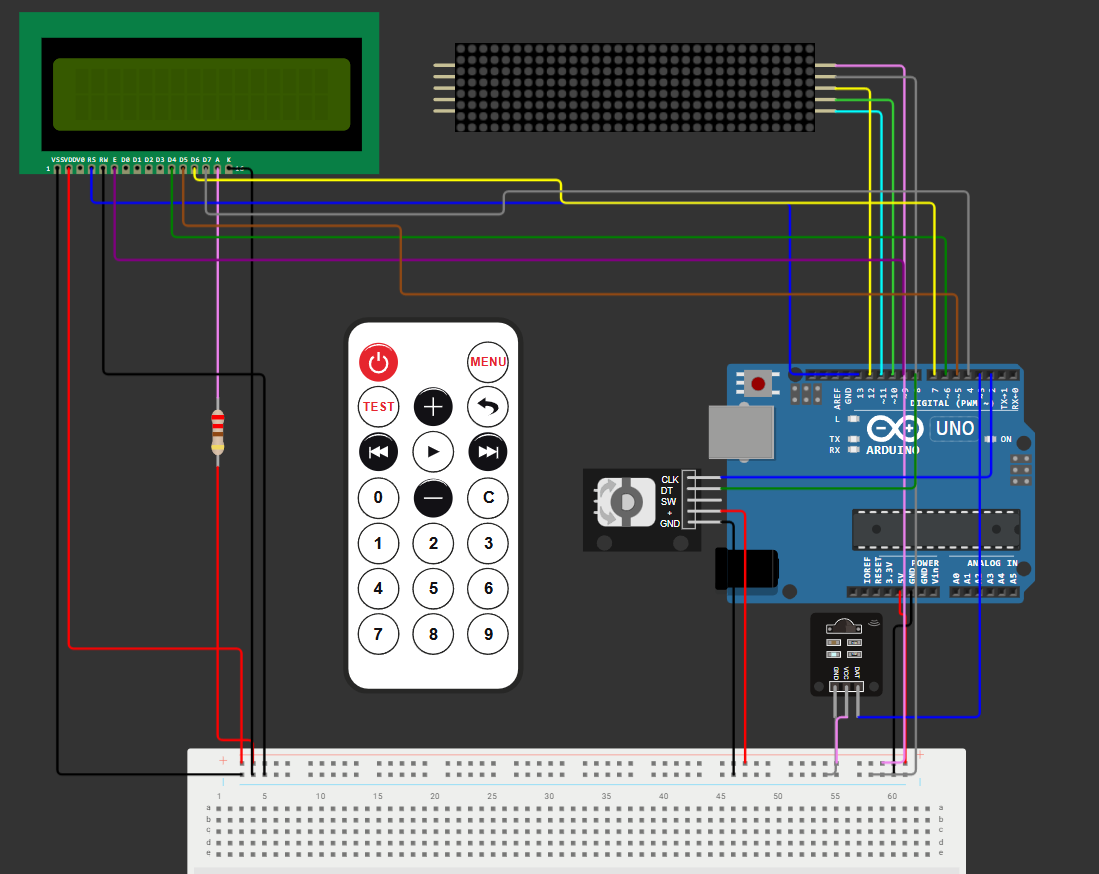
\includegraphics[width=0.8\textwidth]{media/collegamenti.png}
    \caption{Schema di collegamento dei componenti hardware}
    \label{fig:setup-hardware-diagram}
\end{figure}

\subsection{Display a matrice LED (MAX7219)}
\label{subsec:setup-max7219}
Collegamenti tra il modulo MAX7219 e il microcontrollore:

\begin{table}[H]
    \centering
    \caption{Collegamenti Matrix (MAX7219) - Microcontrollore}
    \label{tab:matrix-max7219-connections}
    \begin{tabular}{ll}
        \toprule
        \textbf{Matrix Pin} & \textbf{Microcontrollore Pin} \\
        \midrule
        VCC                 & 5V                            \\
        GND                 & GND                           \\
        DIN                 & Pin 12                        \\
        CS                  & Pin 10                        \\
        CLK                 & Pin 11                        \\
        \bottomrule
    \end{tabular}
\end{table}

\subsection{Display LCD 16x2}
\label{subsec:setup-lcd}
Collegamenti tra il modulo LCD 1602 e il microcontrollore:

\begin{table}[H]
    \centering
    \caption{Collegamenti LCD Display (16x2) - Microcontrollore}
    \label{tab:lcd-16x2-connections}
    \begin{tabular}{ll}
        \toprule
        \textbf{LCD Pin} & \textbf{Microcontrollore Pin}                \\
        \midrule
        RS               & Pin 13                                       \\
        E                & Pin 9                                        \\
        D4               & Pin 6                                        \\
        D5               & Pin 5                                        \\
        D6               & Pin 7                                        \\
        D7               & Pin 4                                        \\
        VSS              & GND                                          \\
        VDD              & 5V                                           \\
        RW               & GND                                          \\
        A (Anodo)        & 5V (attraverso resistenza da 220 \(\Omega\)) \\
        K (Catodo)       & GND                                          \\
        \bottomrule
    \end{tabular}
\end{table}

\subsection{Ricevitore Infrarossi (IR)}
\label{subsec:setup-ir}
Collegamenti tra il modulo ricevitore IR e il microcontrollore:

\begin{table}[H]
    \centering
    \caption{Collegamenti IR Receiver Module - Microcontrollore}
    \label{tab:ir-receiver-connections}
    \begin{tabular}{ll}
        \toprule
        \textbf{IR Pin} & \textbf{Microcontrollore Pin} \\
        \midrule
        VCC             & 5V                            \\
        GND             & GND                           \\
        OUT/Data        & Pin 3                         \\
        \bottomrule
    \end{tabular}
\end{table}

\subsection{Encoder Rotativo}
\label{subsec:setup-encoder}
Collegamenti tra l'encoder rotativo e il microcontrollore:

\begin{table}[H]
    \centering
    \caption{Collegamenti Rotary Encoder Module - Microcontrollore}
    \label{tab:rotary-encoder-connections}
    \begin{tabular}{ll}
        \toprule
        \textbf{Encoder Pin} & \textbf{Microcontrollore Pin} \\
        \midrule
        CLK                  & Pin 2                         \\
        DT                   & Pin 8                         \\
        SW (Switch)          & Non utilizzato                \\
        VCC                  & 5V                            \\
        GND                  & GND                           \\
        \bottomrule
    \end{tabular}
\end{table}

\section{Build del Progetto}
\label{sec:build}
Il progetto può essere eseguito in due modalità: \textbf{simulatore} e \textbf{hardware fisico reale}.\\
Per eseguire il progetto in modalità simulatore il file da eseguire sarà \texttt{src/main.cpp}, mentre per eseguire il progetto su hardware
reale il file da eseguire sarà \texttt{src/main/main.ino}.\\
Questo perché l'IDE di Arduino vuole che il file da iniettare sulla scheda sia contenuto in una cartella con lo stesso nome del file.\\
I file sono identici se non per la riga di codice che definisce se il progetto è in produzione o meno.
\begin{itemize}
    \item \textbf{Simulatore:} \texttt{PRODUCTION = false}
    \item \textbf{Hardware reale:} \texttt{PRODUCTION = true}
\end{itemize}

La differenziazione data da questa riga di codice è necessaria per gestire i codici infrarossi generati dal telecomando nei due ambienti.\\
Infatti, per il simulatore Wokwi, i codici infrarossi sono diversi rispetto a quelli inviati dal telecomando reale.\\
Se si volesse cambiare il telecomando, basterebbe rimappare i codici di production (\texttt{PRODUCTION\_CODES}) nel file \texttt{lib/utils/utils.h}.

\subsection{Struttura del Progetto}
\label{subsec:progetto-struttura}
Il progetto è organizzato seguendo una struttura modulare che facilita lo sviluppo e la manutenzione del codice. \\
Di seguito è riportata la struttura delle directory e dei file principali:\\
\begin{forest}
    for tree={
    font=\ttfamily,
    grow'=0,
    child anchor=west,
    parent anchor=south,
    anchor=west,
    calign=first,
    edge path={
            \noexpand\path [draw, \forestoption{edge}]
            (!u.south west) +(7.5pt,0) |- node[fill,inner sep=1.25pt] {} (.child anchor)\forestoption{edge label};
        },
    before typesetting nodes={
            if n=1
                {insert before={[,phantom]}}
                {}
        },
    fit=band,
    before computing xy={l=15pt},
    }
    [TETRIS\_ARDUINO
    [lib
            [utils
                    [utils.h [{\color{gray}(Libreria utility)}], font=\footnotesize\itshape\color{gray}]
            ]
    ]
    [report [{\color{gray}(Report directory)}, font=\footnotesize\itshape\color{gray}]
            [media [{\color{gray}(Media directory)}, font=\footnotesize\itshape\color{gray}]]
            [report.tex [{\color{gray}(Report in Latex)}, font=\footnotesize\itshape\color{gray}]]
            [report.pdf [{\color{gray}(Report prodotto)}, font=\footnotesize\itshape\color{gray}]]
    ]
    [src
            [{\color{gray}(Source code directory)}, font=\footnotesize\itshape\color{gray}]
            [main
                    [{\color{gray}(Report directory)}, font=\footnotesize\itshape\color{gray}]
                    [main.ino [{\color{gray}(Arduino IDE entry point)}, font=\footnotesize\itshape\color{gray}]]
            ]
            [main.cpp [{\color{gray}(PlatformIO entry point)}], font=\footnotesize\itshape\color{gray}]
    ]
    [diagram.json [{\color{gray}(File di configurazione Wokwi - circuiteria)}, font=\footnotesize\itshape\color{gray}]]
    [platformio.ini [{\color{gray}(File di configurazione PlatformIO)}, font=\footnotesize\itshape\color{gray}]]
    [README.md [{\color{gray}(Documentazione)}, font=\footnotesize\itshape\color{gray}]]
    [wokwi.toml [{\color{gray}(File di configurazione Wokwi - simulatore)}, font=\footnotesize\itshape\color{gray}]]
    ]
\end{forest}
\subsection{Simulatore}
Di seguito sono riportati i passaggi per eseguire il progetto in modalità simulatore.
\begin{enumerate}
    \item Aprire VSCode
    \item Installare l'estensione \href{https://marketplace.visualstudio.com/items?itemName=Wokwi.wokwi-vscode}{Wokwi}
    \item Installare l'estensione \href{https://marketplace.visualstudio.com/items?itemName=platformio.platformio-ide}{PlatformIO}
    \item Aprire la cartella \texttt{tetris-arduino} come progetto PlatformIO all'interno di VSCode
    \item In \texttt{src/main.cpp}, verificare che sia presente:
          \begin{lstlisting}
#define PRODUCTION  false
	      \end{lstlisting}
    \item Dal \textbf{Command Palette} (\texttt{F1}) eseguire \texttt{PlatformIO: Build}.
          Questo genera i file di firmware in \texttt{.pio/build/uno/}.
    \item Controllare il file \texttt{wokwi.toml}, deve essere del tipo:
          \begin{verbatim}
[wokwi]
version = 1
firmware = "percorso del file firmware.hex"
elf      = "percorso del file firmware.elf"
	      \end{verbatim}
    \item Avviare il simulatore con il comando \texttt{Wokwi: Start Simulator} dal \textbf{Command Palette} di VSCode.
    \item Wokwi caricherà automaticamente lo schema contenuto in \texttt{diagram.json} insieme al firmware appena compilato e una nuova finestra interattiva del simulatore verrà aperta.
\end{enumerate}

\subsection{Hardware Reale}
\begin{enumerate}
    \item In \texttt{src/main/main.ino}, assicurarsi che sia presente:
          \begin{lstlisting}
#define PRODUCTION  true
	      \end{lstlisting}
    \item Collegare il microcontrollore al PC
    \item Aprire Arduino IDE
    \item Selezionare la scheda \texttt{Arduino UNO} e la porta COM corretta
    \item Iniettare il codice sulla scheda
\end{enumerate}

\section{Screenshot del Gioco}
\label{sec:screenshot}
Di seguito sono riportati alcuni screenshot del gioco in esecuzione.\\
Durante il gioco il monitor seriale del microcontrollore mostra informazioni utili per il debug, come i codici IR ricevuti e le azioni eseguite.\\

\begin{figure}[H]
    \centering
    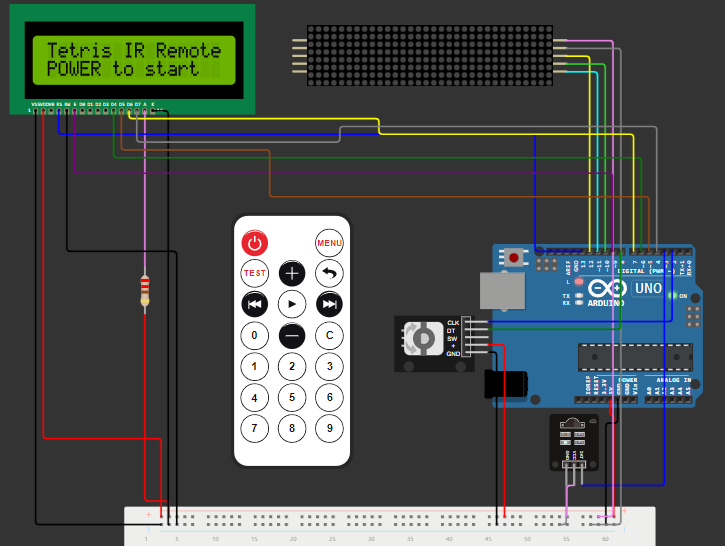
\includegraphics[width=0.8\textwidth]{media/appena_acceso.png}
    \caption{Screenshot del gioco appena acceso}
    \label{fig:appena_acceso}
\end{figure}
\begin{figure}[H]
    \centering
    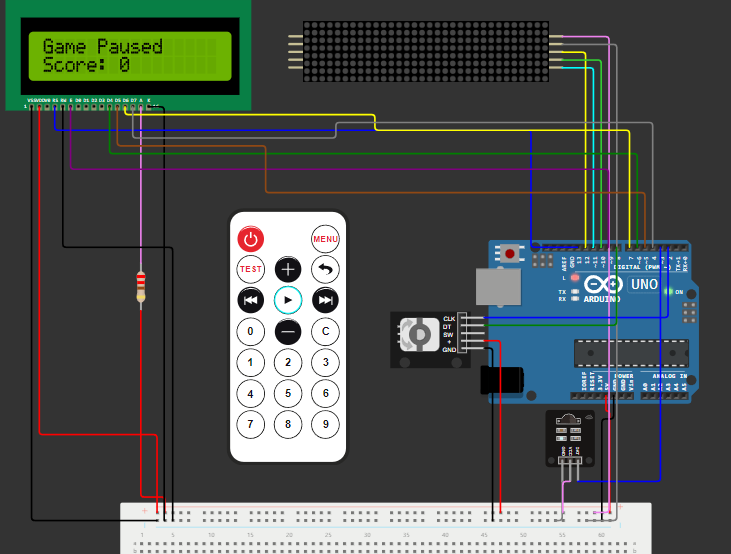
\includegraphics[width=0.8\textwidth]{media/pausa.png}
    \caption{Screenshot del gioco in pausa}
    \label{fig:pausa}
\end{figure}

\begin{figure}[H]
    \centering
    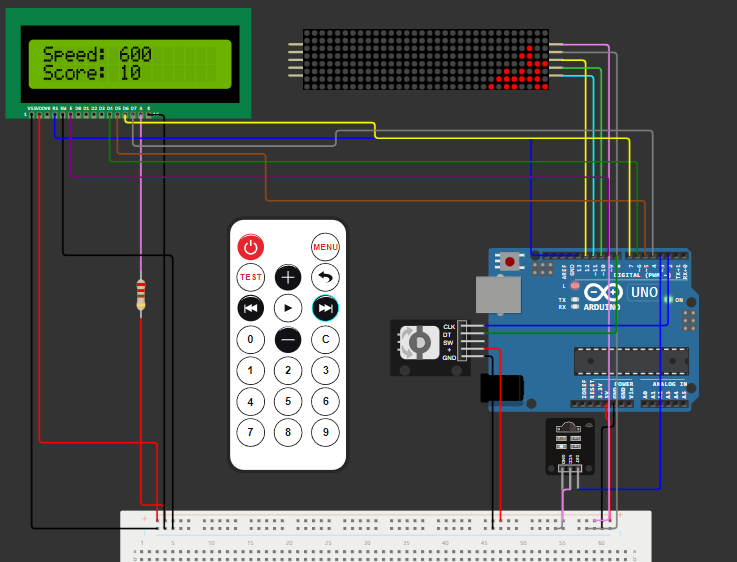
\includegraphics[width=0.8\textwidth]{media/in_gioco.png}
    \caption{Screenshot del gioco in corso}
    \label{fig:in_gioco}
\end{figure}


\begin{figure}[H]
    \centering
    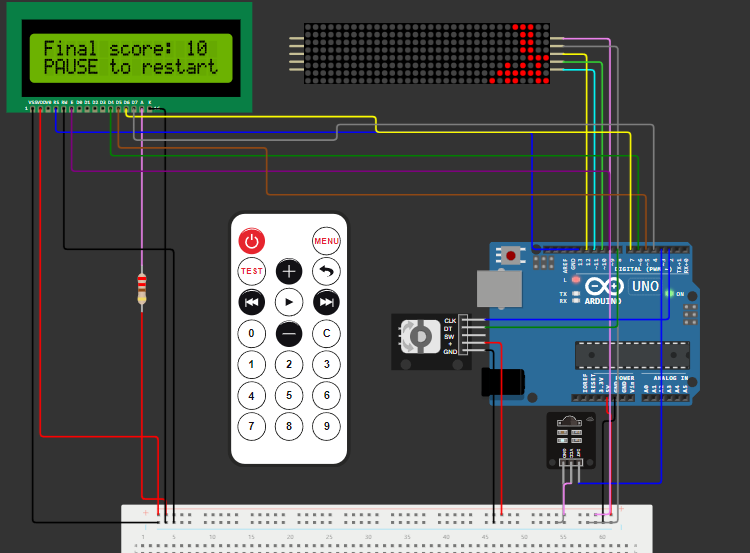
\includegraphics[width=0.8\textwidth]{media/fine_gioco.png}
    \caption{Screenshot del gioco terminato}
    \label{fig:fine_gioco}
\end{figure}


\end{document}